\documentclass[class=../../report, crop=false]{standalone}
\usepackage{graphicx}
\usepackage{caption}
\usepackage[list=true,listformat=simple]{subcaption}
\DeclareCaptionSubType*[alph]{figure}
\captionsetup[subfigure]{labelformat=simple}
\renewcommand\thesubfigure{(\thefigure\alph{subfigure})}

%\DeclareCaptionFormat{cont}{#1 (cont.)#2#3\par}
\begin{document}

\section{Functional Decomposition Diagram} \label{app:funcdecomp}

\begin{figure}[!h]
	\caption{Function Decomposition Diagram}
\end{figure}

\begin{figure}[!htb]
	\ContinuedFloat
	\begin{subfigure}{\textwidth}
		\centering
		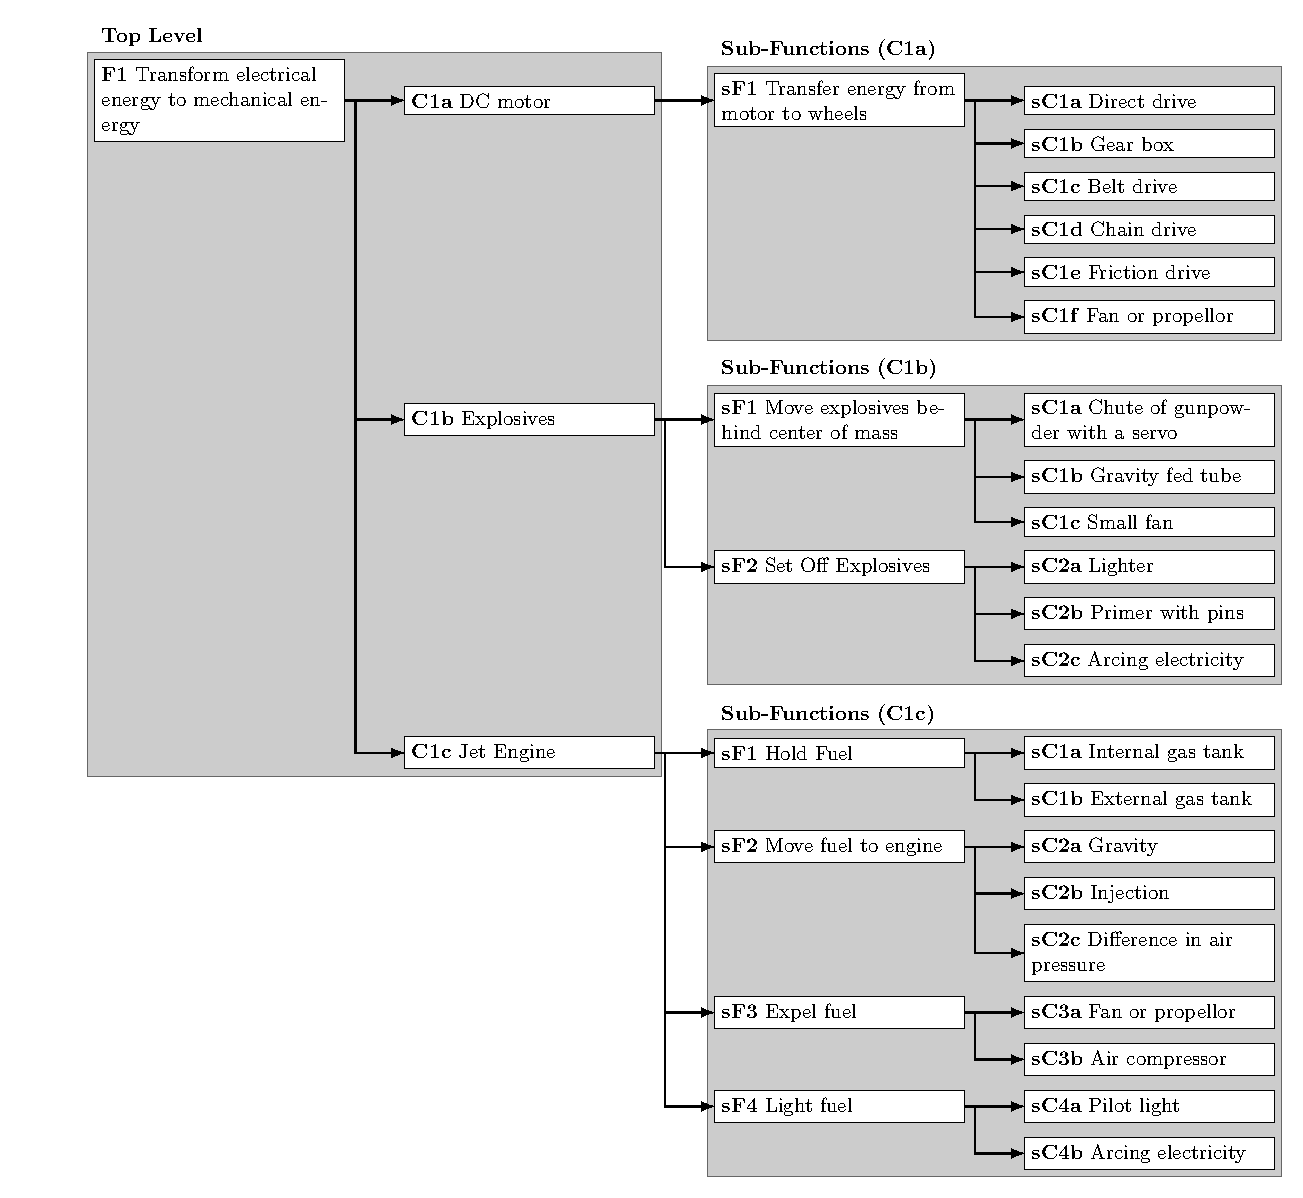
\includegraphics[width=\textwidth]{../../../bin/funcdecomp-1}
		\caption{Functional Decomposition Diagram Part 1}
	\end{subfigure}
\end{figure}

\begin{figure}[!htb]
	\ContinuedFloat
	\begin{subfigure}{\textwidth}
		\centering
		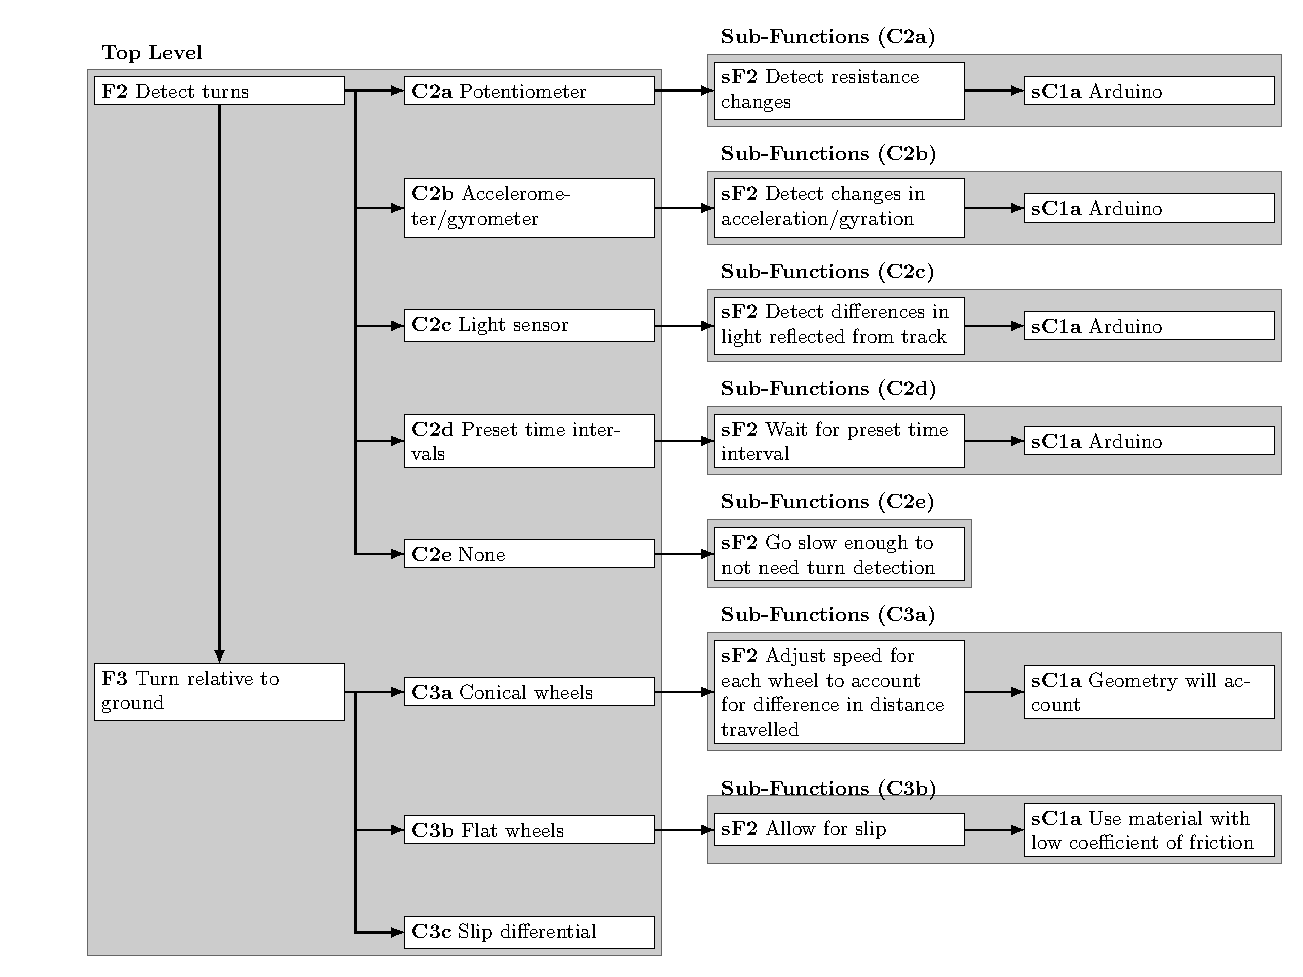
\includegraphics[width=\textwidth]{../../../bin/funcdecomp-2}
		\caption{Functional Decomposition Diagram Part 2}
	\end{subfigure}
\end{figure}

\begin{figure}[!htb]
	\ContinuedFloat
	\begin{subfigure}{\textwidth}
		\centering
		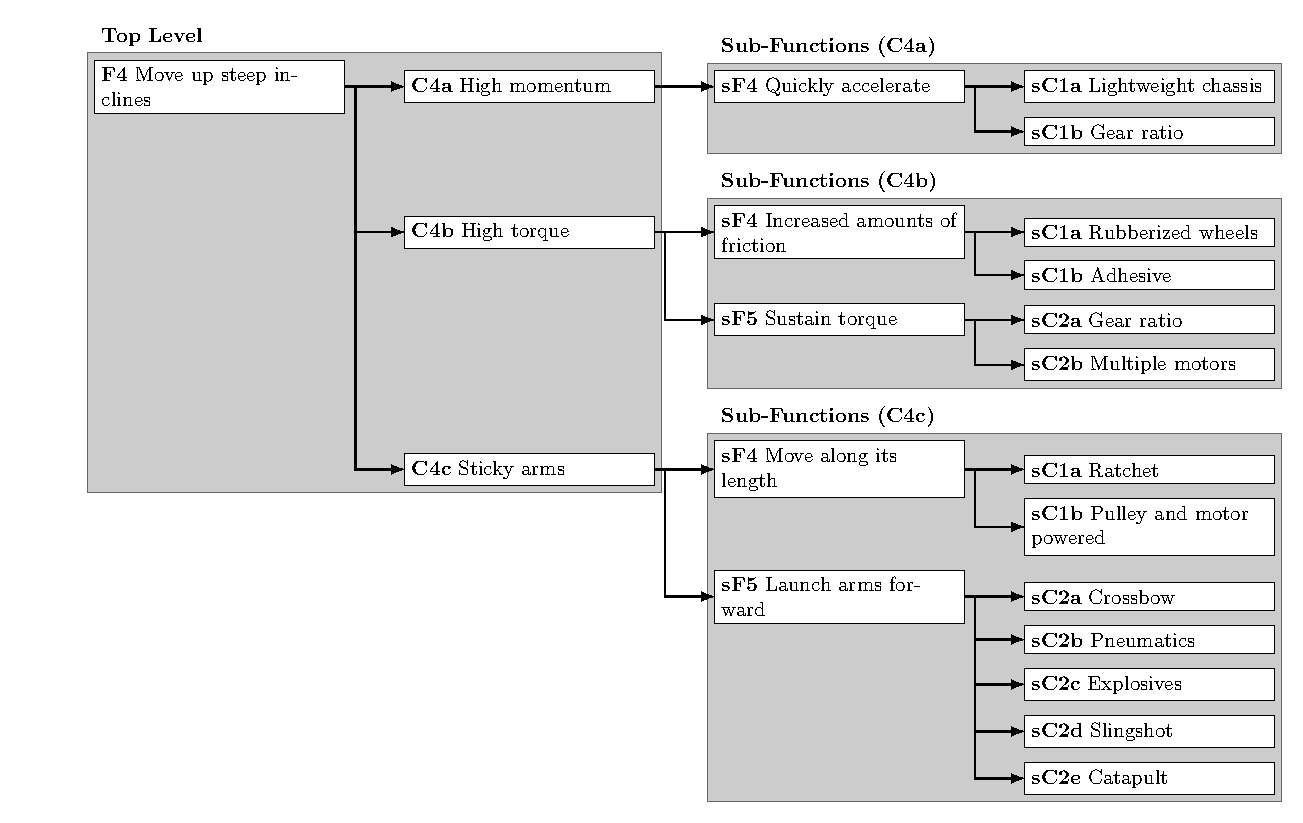
\includegraphics[width=\textwidth]{../../../bin/funcdecomp-3}
		\caption{Functional Decomposition Diagram Part 3}
	\end{subfigure}
\end{figure}

\begin{figure}[!htb]
	\ContinuedFloat
	\begin{subfigure}{\textwidth}
		\centering
		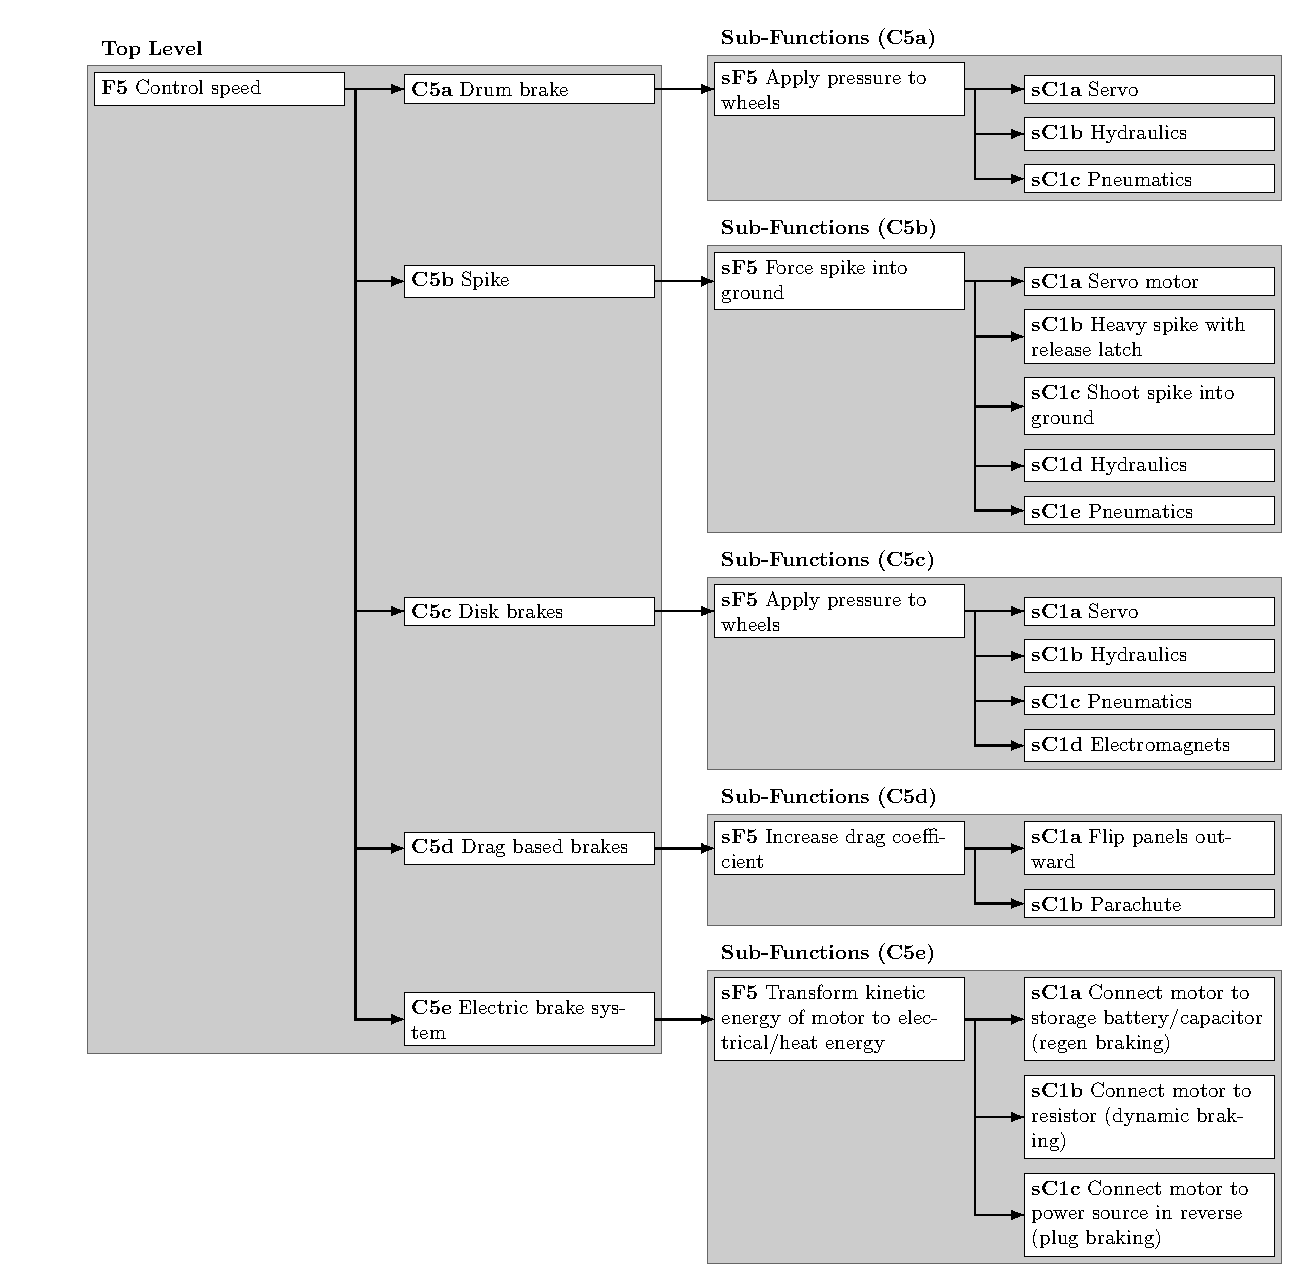
\includegraphics[width=\textwidth]{../../../bin/funcdecomp-4}
		\caption{Functional Decomposition Diagram Part 4}
	\end{subfigure}
\end{figure}

\begin{figure}[!htb]
	\ContinuedFloat
	\begin{subfigure}{\textwidth}
		\centering
		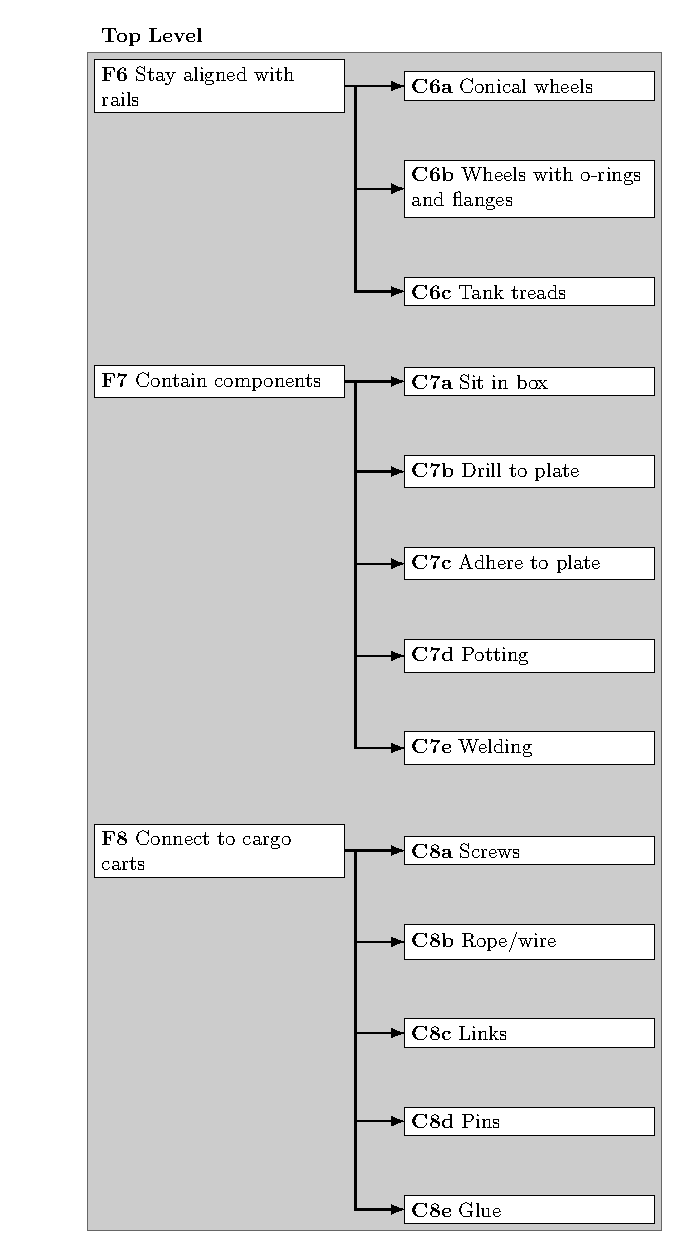
\includegraphics[trim=10.5cm 0 0 0,scale=0.75]{../../../bin/funcdecomp-5}
		\caption{Functional Decomposition Diagram Part 5}
	\end{subfigure}
\end{figure}

\end{document}
